\documentclass{article}
\usepackage{lmodern}
\usepackage{amssymb,amsmath}
\usepackage[T1]{fontenc}
\usepackage[utf8]{inputenc}
\usepackage{upquote}
\PassOptionsToPackage{hyphens}{url} % url is loaded by hyperref
\usepackage[unicode=true]{hyperref}
\hypersetup{pdfborder={0 0 0},
            breaklinks=true}
\urlstyle{same}  % don't use monospace font for urls
\usepackage{longtable,booktabs}
\usepackage{graphicx}
\makeatletter
\def\maxwidth{\ifdim\Gin@nat@width>\linewidth\linewidth\else\Gin@nat@width\fi}
\def\maxheight{\ifdim\Gin@nat@height>\textheight\textheight\else\Gin@nat@height\fi}
\makeatother
% Scale images if necessary, so that they will not overflow the page
% margins by default, and it is still possible to overwrite the defaults
% using explicit options in \includegraphics[width, height, ...]{}
\setkeys{Gin}{width=\maxwidth,height=\maxheight,keepaspectratio}
\usepackage{parskip}
\setcounter{secnumdepth}{0}
% Redefines (sub)paragraphs to behave more like sections
\ifx\paragraph\undefined\else
\let\oldparagraph\paragraph
\renewcommand{\paragraph}[1]{\oldparagraph{#1}\mbox{}}
\fi
\ifx\subparagraph\undefined\else
\let\oldsubparagraph\subparagraph
\renewcommand{\subparagraph}[1]{\oldsubparagraph{#1}\mbox{}}
\fi

% set default figure placement to htbp
\def\fps@figure{htbp}

% Add references
\usepackage[backend=bibtex,
style=alphabetic
]{biblatex}
\DeclareFieldFormat{labelalpha}{\thefield{entrykey}}
\DeclareFieldFormat{extraalpha}{}

\addbibresource{PRESENTER_PROTOCOL_v2.bib}

% Format table of contents
\renewcommand*\contentsname{Table of contents}

\begin{document}
\section*{Presenter Protocol Definition Version 2}

This document contains the definition of the presenter protocol.\\
The basic idea is to define a simple protocol and allow all servers that support a specific version of the protocol version to be remote controlled by any client supporting matching versions.\\
E.g. you can remote control a presentation running on a pc using your smartphone over bluetooth connection using this presenter protocol.

\tableofcontents

\subsection{Latest version of the document}
\label{latest_version}

The latest release of this document can be found on github at the following url: \url{https://github.com/FelixWohlfrom/Presenter-Protocol/releases}

\subsection{Copyright notice}

Copyright © 2018 Felix Wohlfrom. All rights reserved except the following:\\
You are allowed to to share and translate this document for free. You are also allowed to convert this latex file for displaying purpose e.g. to html, pdf or other output formats. In all cases, a link to the original file needs to be present (see \hyperref[latest_version]{latest version of the document}).

All modifications and distribution to this latex file are forbidden, except if they are sent as a \href{https://github.com/FelixWohlfrom/Presenter-Protocol/pulls}{pull request} via github that needs to be accepted by the repository admin.

\subsection{Conventions used in this document}

The key words ``MUST'', ``MUST NOT'', ``REQUIRED'', ``SHALL'', ``SHALL NOT'', ``SHOULD'', ``SHOULD NOT'', ``RECOMMENDED'', ``MAY'', and ``OPTIONAL'' in this document are to be interpreted as described in \cite{RFC2119}.

\subsection{Presenter protocol definition}

The definition contains three major parts: A general introduction, a description of the connection initiation and the definition of the commands that are supported by the protocol.

\subsubsection{General}

Here you find some general definitions that MUST be supported by both client and server if they implement this presenter protocol.

\begin{enumerate}
    \item Data transmission

        \begin{enumerate}
           \item All data transmitted between the server and the client MUST be transmitted using the JSON protocol as in rfc 8259 \cite{JSON}.
           \item In particular, as noted in rfc 8259, the transmission MUST be UTF-8 encoded.
        \end{enumerate}
    \item Message structure

        All transmitted data between the server and the client MUST be packed into so called \emph{messages}.\\
        These \emph{messages} MUST be structured as the following json encoded text:
\begin{verbatim}
{
    "type": <msg_type>,
    "data": <msg_data>
}
\end{verbatim}

        The following values MUST be supported for \emph{\textless{}msg\_type\textgreater{}}:\\
        VERSION\\
        COMMAND

        The \emph{\textless{}msg\_data\textgreater{}} is a string. The content of the string depends on the \emph{\textless{}msg\_type\textgreater{}} and is now described in detail:

\newpage

        \begin{enumerate}
            \item \emph{\textless{}msg\_type\textgreater{}} VERSION
                \label{msg_version}

                The \emph{\textless{}msg\_data\textgreater{}} MUST be a json string having the following structure:
\begin{verbatim}
{
    "minVersion": <min_version>,
    "maxVersion": <max_version>
}
\end{verbatim}

                \emph{\textless{}min\_version\textgreater{}} MUST contain the minimum version of commands that is supported by the current connection.

                \emph{\textless{}max\_version\textgreater{}} MUST contain the maximum version of commands that is supported by the current connection.

                The server or client MUST support all commands that are defined for the range between \emph{\textless{}min\_version\textgreater{}} and \emph{\textless{}max\_version\textgreater{}}, including both boundary values.

            \item \emph{\textless{}msg\_type\textgreater{}} COMMAND
                \label{msg_command}

                The \emph{\textless{}msg\_data\textgreater{}} MUST be a simple string. Valid values for the commands are defined in the chapter ``\hyperref[command_definition]{Command definition}''.
  \end{enumerate}
\end{enumerate}

\subsubsection{Connection initiation}

Once the first client established a connection to the server, the server MUST response with a \hyperref[msg_version]{\emph{\textless{}msg\_type\textgreater{}} VERSION} message.

The client SHOULD now check if the command versions supported by the server and the command versions supported by the client match. If the range of versions supported by the server and the versions supported by the client don't match, the client SHOULD disconnect from the server.

Once the connection is established, the client can send the following commands to the server.

\subsubsection{Command definition}
\label{command_definition}

The following table describes the commands that can be sent using the \hyperref[msg_command]{\emph{\textless{}msg\_type\textgreater{}} COMMAND}.\\
The ``\emph{Command}'' row contains the command, that is sent in the \emph{\textless{}msg\_data\textgreater{}} field.\\ The ``\emph{Min Version}'' row contains the minimum protocol version
that MUST be supported by both server and client to transmit the command.\\
The ``\emph{Max Version}'' row contains the maximum protocol version that MUST be supported by both server and client to transmit the command. The maximum value for this row MAY be updated in newer releases of the presenter protocol.\\
The ``\emph{Description}'' row contains a description of the action the server MUST execute once it receives the command.

\begin{longtable}{lccp{5cm}}
\toprule
Command & Min Version & Max Version & Description\\
\midrule
\endhead
prevSlide & 1 & 2 & Switch to the previous slide of the presentation\\
nextSlide & 1 & 2 & Switch to the next slide of the presentation\\
startPresentation & 2 & 2 & Start the presentation\\
stopPresentation & 2 & 2 & Stop the presentation\\
\bottomrule
\end{longtable}

\subsection{Examples}

In this chapter there are several examples of json messages and an example command flow which shows the commands that are sent between client and server.

\subsubsection{Version messages}

In this message, the server notifies the client that it supports all commands from command version 1 up to command version 3. This means that the server supports commands version 1, 2 and 3:

\begin{verbatim}
{
    "type": "VERSION",
    "data": "{ \"minVersion\": 1, \"maxVersion\": 3 }"
}
\end{verbatim}

This message notifies the client, that only command version 2 and commands version 3 are supported by the server:

\begin{verbatim}
{
    "type": "VERSION",
    "data": "{ 'minVersion': 2, 'maxVersion': 3 }"
}
\end{verbatim}

\subsubsection{Command messages}

This command message is sent from the client to the server to request a switch to the previous slide of a currently running presentation:

\begin{verbatim}
{
    "type": "COMMAND",
    "data": "prevSlide"
}
\end{verbatim}

This command message is sent from the client to the server to continue the presentation on the next slide:

\begin{verbatim}
{
    "type": "COMMAND",
    "data": "nextSlide"
}
\end{verbatim}

\subsubsection{Command flow}

This diagram displays a common information flow between a server and a client.\\
The server is running on a pc, on which the presentation is running. The client is installed on a smartphone and will remote control the presentation.

The client initiates a connection. Then the server sends the supported command versions to the client. Afterwards, the client checks if the versions supported by the client and the versions by the server have a common range of supported versions.

If there is no match between the supported versions, the client disconnects from the server.

If there is a matching version range, the client will send regularly command messages to the server.

Finally, both server and client can close the connection.

This flow is shown in figure \ref{command_flow}.

\begin{figure}
\centering
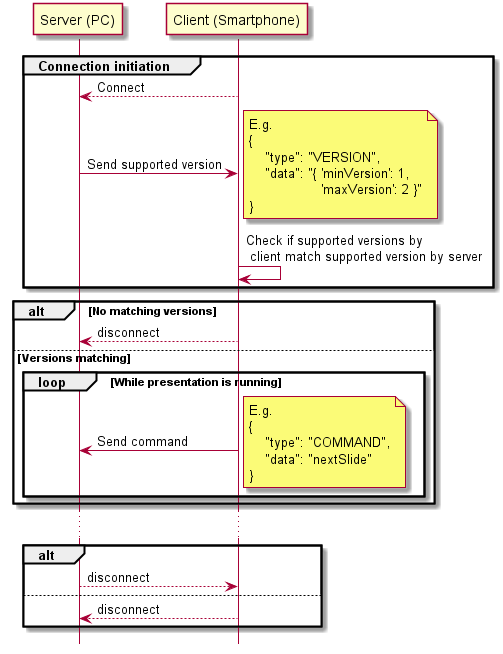
\includegraphics{./diagrams/gen/CommandFlow.png}
\caption{Example command flow}
\label{command_flow}
\end{figure}

\printbibliography[heading=subbibliography]
\addcontentsline{toc}{subsection}{References}

\newpage

\subsection{Changes}

In this chapter you can find the changes that where done in the different releases of the presenter protocol definition.

\begin{longtable}{cl}
\toprule
Version & Changes\tabularnewline
\midrule
\endhead
2 & Added commands to start and stop a presentation\\
1 & First final release \\
  & Converted reference file to latex\\
1 - Draft & Initial version of this document\\
\bottomrule
\end{longtable}

\end{document}
